\capitulo{6}{Trabajos relacionados}

%Este apartado sería parecido a un estado del arte de una tesis o tesina. En un trabajo final grado no parece obligada su presencia, aunque se puede dejar a juicio del tutor el incluir un pequeño resumen comentado de los trabajos y proyectos ya realizados en el campo del proyecto en curso. 

Existe diferentes proyectos que tratan de predecir los brotes de medusas a lo largo de las costas o encontrar que factores son los más determinantes para que estos sucedan.

\section{Articulos}

\subsection{\emph{Deterministic Factors Overwhelm Stochastic Environmental Fluctuations as Drivers of Jellyfish Outbreaks}}

Este grupo de investigación, del que forma parte el Dr.Antonio Canepa, que fue quien nos proporcionó los datos de avistamientos para realizar este proyecto, realizó un estudio sobre los factores más influyentes en los afloramientos de medusas en las costas de Cataluña entre los años 2007 y 2010~\cite{art:ArticuloCanepa_1}.

\subsection{\emph{The jelly report: Forecasting jellyfish using email and social media}}

Se trata de un estudio en el que se recogieron datos de avistamientos a través de las redes sociales y el correo electrónico. Estuvo situado en las costas de Massachusetts,más concretamente, en el cabo de Maine. Se dio una importancia mayor a las direcciones del viento respecto a otras características obteniendo buenos resultados. Una de las teorías aportadas, trataba sobre la presencia de vientos alisios. Estos generan turbulencias en las aguas mas cercanas a las costas, provocando que las medusas no puedan acercase a estas~\cite{articulomedusas2}. Se puede observar un ejemplo en la Figura \ref{articulomedusas2}.
\begin{figure}%[!h]
	\centering
	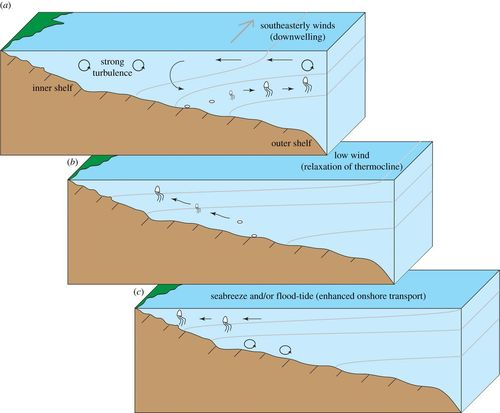
\includegraphics[width=0.55\textwidth]{articuloMedusas2.jpg}
	\caption[Relación entre vientos alisios y medusas]{Relación entre vientos alisios y medusas~\cite{articulomedusas2}.}\label{articulomedusas2}
\end{figure}

\section{Proyectos}

Se han analizado dos tipos de proyectos principalmente: los que unicamente recogen información de avistamientos y otros que realizan predicciones.

\subsection{Perseus}

Se trata de una web en la que podemos registrar los avistamientos que tengamos introduciendo la localización, el tipo de medusa y la densidad de las misma que hay.
Estos registros se pueden consultar desde la misma página.

Web del proyecto: \href{http://www.perseus-net.eu/en/jellyfish_map/index.html}{http://www.perseus-net.eu/en/jellyfish\_map/index.html}

\subsection{NOAA}

Se trata de una web que ofrece una predicción de la bahía de Chesapeake, cercana a Washington DC. Ofrece a través de un mapa coroplético (mapa con áreas coloreadas en distintos colores, que representan diferentes valores de una cierta variable) la probabilidad de la presencia de medusas en cada zona de la bahía.

Web del proyecto: \href{https://ocean.weather.gov/Loops/ocean_guidance.php?model=Sea_Nettles&area=Prob&plot=prob&day=0&loop=1}{NOAA}

\subsection{Infomedusa}

Aplicación para Android y iOS que ofrece información sobre la presencia de medusa en las playas de toda España mediante reportes de informadores asociados.

Web del proyecto: \href{https://infomedusa.es/}{https://infomedusa.es/}

\subsection{MedusApp}

También es una aplicación en la que se recogen reportes de cualquier persona en tiempo real. Un usuario puede informar de la presencia o no de medusas en una playa en la que se encuentre. Estos avisos aparecerán en el mapa al resto de usuarios advirtiendo de la presencia de medusas. También está disponible una versión web.

Aparte de estos avisos, incluye recomendaciones sobre las picaduras y descripciones de las distintas especies de medusas.w

Web del proyecto: \url{http://www.medusapp.net/mapa/}
